

\documentclass[11pt,fleqn]{book} % Default font size and left-justified equations

\input{structure} % Insert the commands.tex file which contains the majority of the structure behind the template
\usepackage{float}

\usepackage{listings} 
\lstset
{ 
    language=C,
    basicstyle=\ttfamily,
    columns=fullflexible,
    keepspaces=true,
    numbers=none,
    stepnumber=1,
    showstringspaces=false,
    tabsize=1,
    breaklines=true,
    breakatwhitespace=false,
    keywordstyle=\color{blue!80!black},
    stringstyle=\color{red!80!black},
    commentstyle=\color{green!40!black},
    morecomment=[l][\color{magenta!80!black}]{\#}
}

\usepackage{caption}
\captionsetup[figure]{font=small,skip=10pt}

%\usepackage{enumitem}
%\setlist{noitemsep} % or \setlist{noitemsep} to leave space around whole list


%%%%% May be too harsh to prevent paragraph breaks across pages! 
%\interlinepenalty 10000
\widowpenalties 1 10000
\raggedbottom


\newcommand{\ilcode}[1]{
    %\vspace{0.5pt}
    \smallskip
    \colorbox{gray!20!white}{
        \centering
        \parbox{\linewidth-2\fboxsep}{
            \lstinline@#1@
        }
    }
    %\vspace{0.5pt}
}

\newcommand{\code}[3]{
    \begin{figure}[]
        \colorbox{gray!20!white}{
            \parbox{\linewidth-2\fboxsep} {
                \centering 
                \lstinputlisting[language=C]{#1}
            }
        }
        \caption{#2}
        \label{#3}
    \end{figure}
}

\usepackage{textcomp}
\usepackage{wrapfig}
\usepackage{float}

\usepackage{silence} % http://ctan.org/pkg/silence
\ErrorFilter{textcomp}{Symbol \textrightarrow not provided}

% Disable paragraph indentation globally since template was indenting some and not others. (looked terrible)
%\setlength{\parindent}{0pt}
%\usepackage[parfill]{parskip}

%\usepackage{showframe}

%%%%%%%%%%%%%%%%%%%%%%%%%%%%%%%%%%%%%%%%%%%%%%%%%%%%%%%%%%%%%%%%%%%%%%%%%%%%%%%%%%%%%%%%%%%%%%%%%
%%%%                                                                                         %%%%
%%%%       Chapter 7:                                                                        %%%%
%%%%                                                                                         %%%%
%%%%%%%%%%%%%%%%%%%%%%%%%%%%%%%%%%%%%%%%%%%%%%%%%%%%%%%%%%%%%%%%%%%%%%%%%%%%%%%%%%%%%%%%%%%%%%%%%

\setcounter{chapter}{7} % Manually adjust chapter counter to number before desired chapter heading

\begin{document}
	
\chapterimage{chapter_head_2.png} % Chapter heading image
\chapter{Implementation of a PI Control System}

\begin{warning}
    \textbf{This lab involves wiring systems with different operating voltages together!} You MUST be careful how you connect things or you will damage either your board or the motor encoder. Read the lab as well as the comments in the template project carefully!
\end{warning}

\setSectionType{Intro}
\section{Control System Implementation}

In the previous lab we modeled a PI controller similar to the one shown in figure \ref{motorPI}. By adjusting the different gain parameters of the proportional and integral portions it is possible to tune the system to respond with smooth and rapid responses to changes in the system's setpoint or load. 

\begin{figure}[tb]
    \centering\includegraphics[width=.9\textwidth]{motorPI.png}
    \caption{Simulink block diagram of a PI control system.}
    \label{motorPI}
\end{figure}

This lab explores implementing a similar control system using software on the STM32F0. Unlike the model, software-driven systems exhibit some limitations that require some adaption from the traditional control system equations. 

\subsection{Discrete-Time Control}

The Simulink model that you created in the previous lab operated in \textit{continuous-time}. This is evident by the use of the Laplace transform to solve the transfer function and represent the integration in the PI controller. Continuous-time systems have a theoretically infinite time resolution, i.e. there is no minimum unit of time that can not be divided further where a result can't be calculated. Many mechanical and analog electronic systems (such as op-amps) are examples of real-world continuous-time systems. 

In contrast, \textit{discrete-time} systems operate only on periodic intervals. This involves the same concepts as quantization and Nyquist sampling rates introduced in the analog lab. A computer cannot monitor an input at every instant of time, rather it periodically samples its input values, calculates a result and then updates the output. Similarly a computer simulation cannot generate results for an infinite number of sample points as well. Simulink approximates a continuous system by using small enough time intervals that they appear continuous. It also rescales this interval when zooming onto portions of the output result for increased resolution. 

Because continuous systems continuously monitor and react to changes in their inputs, they are more responsive than discrete-time systems that only react once after sampling. If a continuous Simulink model were adapted to discrete-time, you would see a significantly worse response than previous, due to the fact that it adjusts on comparatively slow time intervals. Within this lab you will see similar effects caused by how often the PI control loop is run as well as the sampling rate of the motor speed.  

\subsection{Fixed-Point Numbers}
One of the major complications of this lab is that our measured motor speed and error signals are unlikely to result in integer values once converted to meaningful units. The easiest solution is to use floating-point numbers, however this has the disadvantage of introducing large libraries and slow execution. 

In lieu of using floating-point, this lab will use a \textit{fixed-point} number representation. Standard binary integers assign a power-of-two value to each bit, the 0\textsuperscript{th} bit has the value of $2^{0}$ (1), the first has the value $2^{1}$ (2) and so on. In fixed-point, a virtual decimal point is placed in a known position in the variable's bits. Any bits above the decimal point represent integer values, the others below represent fractional values with their values representing $2^{-1}$ (0.5), $2^{-2}$ (0.25) and so on...
Fixed-point is a bit trickier to use with because you manually interpret what is integer and fractional. However, it requires standard integer math operations while giving sub-integer results. 


\subsection{Discrete Integrals}

When converting a modeled PI controller into code, the proportional portion is fairly straightforward. $(output = error * gain)$ However the concept of an integrator isn't one that easily fits into a simple equation at first glance. To do this we must first introduce a small portion of discrete math.

\begin{equation*}
H(t) = K_{i}\int_{0}^{t}e(\tau)d\tau \quad \rightarrow \quad H(s) = K_{i}\left(\frac{1}{s}\right) \quad \rightarrow \quad H[z] = K_{i}\left(\frac{1}{1-z^{-1}}\right)
\end{equation*} 


\noindent The above equation shows both the continuous (s-domain) and discrete (z-domain) transfer functions for an integral with gain. The basic concept of an integral is to measure the area under a curve, ideally at infinite resolution. One simple way to approximate an integral is to use a \textit{Riemann sum} which places a series of rectangles under the curve and then sums the area of all the rectangles together. 

If you think back to the analog lab, it is possible to digitize an arbitrary analog waveform by quantizing it; essentially rebuilding the signal as a series of rectangles where the height of each rectangle is the value in consecutive values of an array or data stream. A first-order discrete integral is very much the same concept and is in fact a Riemann sum. By summing each of the samples together a rough integration process occurs. As positive samples are summed, the larger the integral value will grow. Likewise, the negative samples that appear decrease the accumulated value or even turn it negative. 

\begin{figure}[tb]
    \centering\includegraphics[width=.8\textwidth]{riemann.png}
    \caption{Example of quantization and how it is used in a Riemann sum to approximate a discrete-time integral.}
    \label{riemann}
\end{figure} 

Knowing this it is simple to represent a discrete first-order integral in the following form:
\begin{equation*}
y[n] = y[n-1] + (K_{i} * x[n])
\end{equation*} 
\noindent Where $y[n]$ is the new value of the integral, $y[n-1]$ is the previous value, $K_{i}$ is the integral gain and $x[n]$ is the new input value. 

\setSectionType{STM32F0}
\section{Using the H-Bridge and DC Gearmotor}

For this lab we will be using the Polulu 2824 - 50:1 Gearmotor. It is a 12-volt brushed DC motor with a maximum speed of 200 RPM (rotations-per-minute) after the 50:1 gearbox on the output shaft. The motor shaft has a 64-count quadrature encoder which we will be using to measure the motor speed. 

Although it is a 12-volt motor, you will be running the motor on only 6-volts. This is to protect both the motor and the H-bridge from high current burnout if the motor were to be stalled (stuck).


\begin{figure}[tb]
    \centering\includegraphics[width=.5\textwidth]{motor.png}
    \caption{Polulu 2824 - 50:1 Gearmotor}
    \label{motor}
\end{figure}

\subsection{Connecting the Motor}
Figure \ref{labeled_pinout} shows an annotated pinout of both the motor connector (referenced by wire color) and the reference H-bridge board. If you are using your own board design make sure that your pinout matches the motor connector, otherwise you'll have to connect using jumper wires. On the reference H-bridge board, the blue labeled pins are where you will want to plug the motor cable in.

\begin{warning}
    When connecting the motor to the H-bridge board make sure not to reverse the connector. This will swap power and ground on the encoder and may destroy it!
\end{warning}

\begin{figure}[t]
    \begin{center}
        \hspace*{-3.4cm}
        \includegraphics[width=0.8\paperwidth]{labeled_pinout.png}
        \caption{Pinout of the H-Bridge reference board and motor cable.}
        \label{labeled_pinout}
    \end{center}
\end{figure}


\subsection{Connecting the H-Bridge to the Discovery Board}
The L298 has three inputs that we'll need to connect to the STM32F0. These are described in it's datasheet as ``IN 1'', ``IN 2'' and ``EnA''. In figure \ref{labeled_pinout}  as well as the operation table below I reference them as ``DIR A'', ``DIR B'' and ``ENABLE'' (labeled in Brown) since those names describe their function more clearly.

The key feature of an H-bridge circuit is that it allows the controller to run the motor in both directions. By changing the polarity of the two ``DIR'' pins, the user can select the direction that the motor turns. Figure \ref{hbridge} shows how the L298 (H-bridge) drives the motor according to its inputs.

\begin{figure}[b]
    \centering\includegraphics[width=.8\textwidth]{hbridge.png}
    \caption{Control settings for the H-Bridge.}
    \label{hbridge}
\end{figure}

For this lab we'll want to avoid using the electronic brake feature. This is because the gearbox has enough inertia that hard-stopping the motor using the motor windings is not only overkill, but puts a good deal of stress on the motor that we don't need. Likewise, don't ever change the motor direction without stopping it first! 

\subsection{PWM and the H-Bridge}
Because of the stress the electronic brake would cause to the motor, it isn't a good idea to use it (or the direction pins) to control the motor speed. Instead a more appropriate method is the H-bridge enable pin, when this pin is low the driver is disabled and essentially disconnected from the motor. In this state it doesn't try to stop the motor (unlike the electronic brake), it simply isn't providing any more power.

\noindent By connecting the enable pin to a PWM output, we'll get a very similar output signal from the H-bridge. This amplified PWM signal approximates driving the motor with an analog voltage. In order to stop the motor completely, simply hold the enable pin low long enough that the motor stops turning. 

\subsection{Quadrature Encoders}

Digital encoders are devices that output a series of pulses as the motor shaft rotates. By measuring the time between pulses or counting how many pulses arrive within a time period it is possible to determine the speed of the motor shaft. Quadrature encoders get their name because they output quadrature-phase signals that are 90° out of phase with each other. By looking at what signal leads (rises first) the other it is possible to tell the direction that the motor is rotating. Figure \ref{quadrature} shows an example of two quadrature-phase signals that will resemble the output of the encoder used in the lab.

\begin{figure}[tb]
    \centering\includegraphics[width=.6\textwidth]{quadrature.png}
    \caption{Example of quadrature-phase signals.}
    \label{quadrature}
\end{figure}

\noindent While it is possible to count/measure the encoder signals manually, the more complex timers in the STM32F0 have an encoder input mode that directly accepts quadrature signals. When configured, the timer value is becomes a counter that increments upwards or downwards each time the encoder delivers a pulse. Figure \ref{encoder} from the peripheral manual shows example quadrature signals and how the timer value changes.

\begin{figure}[tb]
    \centering\includegraphics[width=.9\textwidth]{encoder.png}
    \caption{Demonstration of the timer's value using quadrature encoder mode during motor operation. }
    \label{encoder}
\end{figure}

The specific encoder that we have on the motor for this lab is a 64-count device. This means that there are 64 pulse transitions for every rotation of the motor shaft. Because our motor has a 50:1 gearbox on it, this means that a single rotation of the external output shaft results in 3200 pulses. In order to get the full 200 RPM output (not possible on 6v) then theat the internal motor must spin at 10000 RPM which giving us 650000 encoder pulses per second. 

While 640-thousand might sound like a lot of pulses, it isn't very much when you consider that we'll want our control loop to run at frequencies much faster than a second. Because we want to reduce the amount of decimal math, you will want to choose a sampling rate that results in an integer ratio between encoder count and output RPM. This task is explored in section \ref{encoder_example}.

\section{Connecting the Encoder}
While the other pins connecting the H-bridge board to the STM32F0 have all been processor outputs (inputs to H-bridge) the encoder pins are processor inputs. Because the encoder will be operating at 5V, the outputs of the encoder will be outputting 5V. This means that whatever pins we use to connect the encoder must be 5V tolerant!

\subsection{5V Tolerant GPIO Pins}
Luckily, the 3V STM32F0 processor happens to have a number of 5V tolerant pins. Shown in figure \ref{pinTypes} and in the STM32F072R8 datasheet, table 12 lists the different I/O structures and their capabilities.  

\begin{figure}[tb]
    \centering\includegraphics[width=.9\textwidth]{pinTypes.png}
    \caption{I/O structure types for GPIO pins on the STM32F0. The 5V tolerant types have been circled.}
    \label{pinTypes}
\end{figure}

Table 13, shown in figure \ref{pins} has a column indicating the I/O structure for each pin. Make sure when you are selecting input pins for the encoder interface that they are either of I/O structure type ``FT'' or ``FTf'' otherwise you'll fry the STM32F0!

\begin{warning}
    Check the pin I/O structure type, before applying any power to the system. \textbf{You must be using 5V tolerant pins for the encoder inputs!} 
\end{warning}



\begin{figure}[tb]
    \centering\includegraphics[width=.9\textwidth]{pins.png}
    \caption{Column indicating I/O structure type for pins.}
    \label{pins}
\end{figure}

\subsection{Determining the Encoder Sampling Rate} \label{encoder_example}

Our motor's quadrature encoder has 64 counts per (internal) motor shaft revolution. With the 50:1 gearbox, the motor has a maximum output rate of 200 RPM which requires the internal motor shaft to rotate at 10000 RPM resulting in 640000 encoder counts per minute. For this lab we'll be using a timer interrupt to periodically measure the value of the encoder interface to determine the output speed of the motor. However, this timer interrupt won't only be calculating the speed of the motor but also running the PI control loop.

When choosing the sampling rate of the encoder, the shorter we make the period between interrupts (higher interrupt frequency) the less time we have to accumulate encoder counts for a given motor speed. In comparison, the longer the period between interrupts the more encoder counts we accumulate. 
Because we are also using this interrupt to operate the PI control loop we end up with a trade-off, faster interrupts mean a faster responding PI system but also means that we get a more granular measurement of the motor speed. Slower interrupts give better speed resolution but worse PI response.

When determining an appropriate speed for this lab, you'll probably want something less than a 50mS period between interrupts (20Hz, good speed resolution, bad PI response), but not anything smaller than 10mS because your encoder output will be too granular to be useful. Because we want to avoid most decimal math, we need to choose an interrupt rate that gives an integer ratio between the encoder count and the motor speed. Because typically your encoder counts per minute won't divide evenly into seconds, it can become a bit inconvenient to solve things in terms of frequency. An easier approach is to work in terms of the period between encoder counts. Since decimal values of a second can be directly converted into smaller time units, it's far easier to derive PSC (prescalar register) and ARR (auto-reload register) values to give you the desired delay between timer interrupts.


\subsection{Example: Solving for an Appropriate Sampling Rate}

Using the maximum motor rate rate of 200 RPM (10000 RPM internal shaft) and 640000 counts/minute we know that the period between each encoder count/pulse is (1/640000)\textsuperscript{th} of a minute. Multiplying this by 60 to get the value in seconds gives (60/640000)\textsuperscript{th} of a second. 
At this point you will want to decide what ratio you want there to be between encoder count and output RPM. For example, if you have a ratio of 2:1 then for a speed of 200 RPM you would receive 400 encoder counts. This means that each encoder count represents a resolution of 0.5 RPM on the output. A ratio of 1:1 would give you only a resolution of 1 RPM, a ratio of 4:1 gives you 0.25 RPM. 

This example will use a ratio of 5:1 which results in a interrupt period that is FAR too slow to use for a PI controller, but has excellent speed resolution. While these calculations won't be useful for an actual system, they will demonstrate the concept of how to calculate things out. 

With a ratio of 5:1 we receive 1000 encoder counts per timer interrupt period at an output speed of 200 RPM. Since we know the period between encoder counts, we can multiply that value to find the desired interrupt period. $(60/640000)*1000 = (60000/640000) = 0.09375$ seconds (93.75mS or 93750uS)

Now that we know what the timer period we want between timer interrupts, derive PSC and ARR values that give us the appropriate delay. As demonstrated in the timers lab, a simpler way to derive these values is to use the prescaler to get the timer counting at the base unit of time that your period is in. For the above example, the decimal seconds value can be rounded with reasonable accuracy into an integer micro-second value. If using the prescaler to cause the timer to count in micro-seconds (8Mhz/8 = 1Mhz) then all that is required is to count 93750 timer tic's with the ARR value to get the desired period. 

Although counting to 93750 with a 32-bit timer isn't hard, this lab uses a 16-bit timer which can't count that high. Because the target is out of range at the current timer frequency (1Mhz, 1uS period) then we can increase the prescaler to cause the timer to count slower, giving us a larger time range before hitting the end of the timer. In the case of the above example, lets increase the prescaler so that we have a period of 2uS (500kHz) between every timer tick. Because each tick takes twice as long, we only need to count half as many of them as previous. This gives us (93750/2) = 46875 timer tics which is within the range of the 16-bit timer.

In summary: for a 5:1 ratio between encoder count and output RPM
\begin{itemize}
    \item 16-bit timer PSC = 15 
    \item 16-bit timer ARR = 46875
    \item Timer Interrupt Period: 93.75 mS or 10.666 Hz
\end{itemize}


\section{STMStudio Real-Time Viewer}

\begin{wrapfigure}{R}{0.2\textwidth}
    \centering\includegraphics[width=0.15\textwidth]{studioicon.PNG}
\end{wrapfigure}

While it is possible to view and edit variables using the debugger interface in {\textmu}Vision, it has a number of limitations that make it inconvenient to edit parameters on the fly. Likewise, Kiel doesn't have any way to plot how variables change in real-time as a system is running. Because of this we'll be using another tool called STMStudio to view and tune the performance of our PI controller. 

\noindent For simplicity, we'll be using a configuration file for STMStudio which sets up the variable viewers and some display equations. You can find it with the code template provided in the lab materials. To load a saved configuration use the ``open'' option from the file menu or the toolbar icon.


\begin{figure}[tb]
    \centering\includegraphics[width=.5\textwidth]{loadConfig.png}
    \caption{Loading the configuration file.}
    \label{loadConfig}
\end{figure}

After loading the configuration file the program should complain about a missing executable file. This is because it's looking for the binary .ELF file that was used while saving the configuration. ELF files are containers for the machine-language program binary that gets programmed onto the STM3F0. After compiling the template project, you'll be able to connect STMStudio to your compiled .ELF file using the ``Import variables'' option from the file menu or the toolbar icon.




\begin{figure}[tb]
    \centering\includegraphics[width=.5\textwidth]{loadExec.png}
    \caption{Loading the binary executable file.}
    \label{loadExec}
\end{figure}


Afterward the window shown in figure \ref{confExec} should open. Select the ellipses button next to the "Executable file" edit box. You'll want to find and select the compiled .ELF file that {\textmu}Vision generates when you build the project. After loading the .ELF file, close the import window.

\begin{warning}
Although Kiel {\textmu}Vision generates ELF-type files for programming the STM32F0, it saves them in the project directory with an .AXF file extension. This file can be found in the ``<project folder>/MDK-ARM/<project name>/'' directory. Make a copy and rename the file extension to .ELF for use with STMStudio. 
\end{warning}
% (Should be at: <workspace>/<project_folder>/debug)




\begin{figure}[tb]
    \centering\includegraphics[width=.8\textwidth]{confExec2.png}
    \caption{Selecting the path to the .ELF binary executable file.}
    \label{confExec}
\end{figure}

\noindent Because STMStudio doesn't try to program the board with your code, you'll need to load the application using {\textmu}Vision. Because STMStudio connects to the STM32F0 using the ST-Link debugger, you will not be able to run a debugging session within the Kiel toolchain while using STMStudio. 

\noindent Afterward select the ``Start'' option from the run menu in STMStudio or use the toolbar icon that looks like a green play symbol. If it gives you an error about not being able to connect to the STLink, then you probably have the debugger in {\textmu}Vision running. Assuming that everything is set up correctly, the graphs in the variable viewers should start updating. Naturally you can stop the connection by using the stop option that replaces the start while running.

STMStudio also lets you edit parameters while the system is running. On the left-hand panel of the window select the ``Write Variables'' tab shown in figure \ref{writeVars}. In here we've imported the gain parameters as well as the target speed so you can edit them. Click on the "Written Value" column, type a new value and press enter. Typically the write process is fairly quick, although sometimes STMStudio will hang for a moment until it manages to complete. One annoyance is that STMStudio doesn't update the value in the ``Written Value'' column. If something else changes the variable value the edit area won't update to show it. 


\begin{figure}[tb]
    \centering\includegraphics[width=.8\textwidth]{writeVars.png}
    \caption{Adjusting variables in real-time using STMStudio}
    \label{writeVars}
\end{figure}

STMStudio's connection can persist across STM32F0 resets, if you need to reset the processor for some reason you don't have to disconnect first.


\newpage
\setSectionType{Exercise}
\section{Lab Assignment: Implementation of a PI Controller}

This lab exercise is to write a program performing the following tasks:
\begin{itemize}
    \item Tracks motor speed through a quadrature encoder.
    \item Generates a variable duty-cycle PWM signal to drive the H-bridge.
    \item Uses a PI control loop to tune the duty-cycle to achieve the desired speed.
\end{itemize}

\subsubsection{Testing the H-Bridge}
This lab depends on external components that you may need to check-out or purchase from the ECE stockroom:
\begin{itemize}
    \item Jumper wire kit
    \begin{itemize}
        \item There may be jumper wires available from the TA, but kits are available in the stockroom for purchase.
    \end{itemize}
    \item Polulu Gear Motor 
    \begin{itemize}
        \item You'll want to check this out from the digital lab window, ask for the motor for the embedded systems class
    \end{itemize}
    \item H-Bridge Board
    \begin{itemize}
        \item Hopefully your board you designed for Homework 1.4 operates correctly. If not, then there are a limited number of boards available from the TA.
    \end{itemize}
\end{itemize}
Before starting on code development you should connect the motor system together and test to see if the H-bridge is operational. You can test the H-bridge by manually wiring the direction and enable pins to 3V or GND. Use the table in figure \ref{hbridge} to select a direction of rotation and enable the output, the motor should begin rotating once power is applied. 

\begin{warning}
    \textbf{Be careful not to connect the motor connector backwards!} If you do, you'll reverse power and ground on the quadrature encoder. Most devices aren't designed for this condition and you'll likely fry it.
\end{warning}
Figure \ref{system} shows an example of what your complete wiring setup might look like. Take care when selecting encoder input pins, the encoder is powered with 5V. If you don't connect its output to 5V tolerant pins you'll damage the STM32F0.

\begin{figure}[tb]
    \centering\includegraphics[width=.8\textwidth]{system.png}
    \caption{Connected Discovery board, H-bridge, and motor.}
    \label{system}
\end{figure}

\subsubsection{Using the Template Code}
Because of time limitations at the end of the semester, this lab provides partially-complete template code. These template files provide most of the background infrastructure such as the encoder interface.

Your goal is to complete the program by filling in portions of missing code according to instructions given in the comments. Typically in larger code projects it's a bad idea to put all of the functions in the \textit{main.c} file. (gets too big and disorganized) This lab splits the motor control code into a couple of separate files: \textit{motor.h} and \textit{motor.c}. These files are available on the assignment page for download, you will need to include them in your {\textmu}Vision project.

\begin{description}
    \item[main.c] -- Replace the original main.c in your project with this file.
    \item[motor.h] -- This file exports function prototypes to the main application.
    \item[motor.c] -- This file contains motor and control system specific functions. These functions are exposed to the main application through \textit{motor.h}. 
    \item[lab8.tsc] -- This is a STMStudio configuration file that sets up variable viewers and display equations.
\end{description}

\section{Lab Assignment: Tuning the Controller}

After you get the different pieces of the PI controller operational, it's time to tune the gain parameters to improve performance. Using what you know about the different parameters from the control system modeling lab adjust and view the system response using STMStudio for the following scenarios:

\begin{itemize}
    \item Speed change from 0 to 80 RPM
    \item Speed change from 80 to 50 RPM
    \item Speed change from 50 to 80 RPM
    \item Speed change from 80 to 0 RPM 
\end{itemize}
To make things a bit easier the code template uses the user-button to toggle and switch around to the different speeds required. You can manually edit the target speed using STMStudio or the debugger but pressing the button should cycle between all the required scenarios. 

%\begin{figure}[tb]
%    \centering\includegraphics[width=.9\textwidth]{tuning1.png}
%    \caption{}
%    \label{tuning1}
%\end{figure}

%% Full-width figure


Some examples of a moderately-tuned PI controller are shown in figures \ref{tuning1} to \ref{tuning3}. Having an adjusted system will cause the motor to speed up much faster than when it was un-tuned. Remember that the motor requires takes a while to slow down, and that there isn't any way to instantly stop without using electronic braking. This means that transitions to slower speeds aren't easily adjusted to increase the fall rate. 

%\begin{figure}[tb]
%    \centering\includegraphics[width=.9\textwidth]{tuning2.png}
%    \caption{}
%    \label{tuning2}
%\end{figure}

%% Full-width figure


We don't expect perfection with the tuning of your system. As long as you have a reasonable performance increase over a un-tuned system it will be sufficient. (Operation as shown in figures \ref{tuning1} to \ref{tuning3} is acceptable.) Because it's difficult to stop and capture screenshots from STMStudio, you won't be required to include graphs in your postlab report. However, you'll need to keep track of what parameters you used and describe the behavior of the system. 
\begin{figure}[b!]
    \begin{center}
        \hspace*{-3.4cm}
        \includegraphics[width=0.8\paperwidth]{tuning1.png}
        \caption{Setpoint/Target transition from 0 to 80 RPM. Motor speed is shown in blue, setpoint in red, and PWM duty-cycle in purple. }
        \label{tuning1}
    \end{center}
\end{figure}

\begin{figure}[]
    \begin{center}
        \hspace*{-3.4cm}
        \includegraphics[width=0.8\paperwidth]{tuning2.png}
        \caption{Setpoint/Target transition from 80 to 0 RPM. The motor requires a significant amount of time to stop even though the drive PWM is completely off. }
        \label{tuning2}
    \end{center}
\end{figure}

%\begin{figure}[tb]
%    \centering\includegraphics[width=.9\textwidth]{tuning3.png}
%    \caption{}
%    \label{tuning3}
%\end{figure}

%% Full-width figure
\begin{figure}[]
    \begin{center}
        \hspace*{-3.4cm}
        \includegraphics[width=0.8\paperwidth]{tuning3.png}
        \caption{Setpoint/Target transition from 80 to 50 RPM. Notice the undershoot and recovery on the transition}
        \label{tuning3}
    \end{center}
\end{figure}

%
%
%
%
%\setSectionType{Intro}
%\section{Control System Basics}
%
%
%%\begin{figure}[tb]
%%    \centering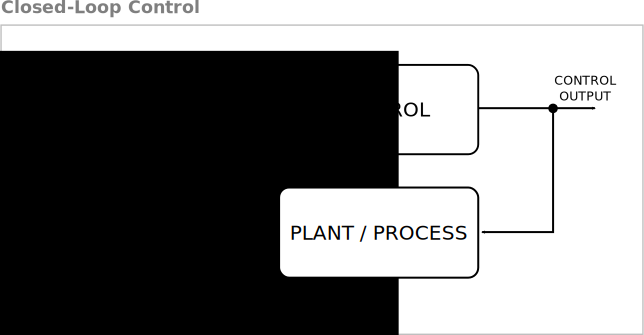
\includegraphics[width=.8\textwidth]{control_block}
%%    %\parbox{.75\textwidth}{\caption{Basic closed-loop control system. The output from the control block is fed into the physical ``plant'' and the generated output is compared against the target input.}}
%%    \caption{Basic closed-loop control system.}
%%    \label{control_block}
%%\end{figure}
%
%\subsection{PID Control Systems}
%The acronym PID represents the three mathematical relations used within the control system; and stand for proportional, integral, and derivative. PID controllers are commonly used in industrial systems because they offer rapid error correction, good stability and can be tuned to react properly to the unique characteristics of a specific system.
%
%The overall equation of a PID control system can be modeled by the following equation, where $c(t)$ represents the output control, and $e(t)$ the input error. 
%
%    \begin{equation*}
%    c(t) = K_{p}e(t) + K_{i}\int_{0}^{t}e(\tau)d\tau + K_{d}\frac{de(t)}{dt}
%    \end{equation*} 
%
%The outputs of each portion (proportional, integral, derivative) are combined to form the control signal fed to the system plant. The PID controller is tuned by adjusting scaling coefficients for each of these. Each of the three portions can be used in isolation to make simpler control systems. The following sections describe the effect each of the mathematical relationships has on the control signal depending on the input error. 
%
%%A PID controller continuously calculates the system error from the input setpoint and feedback from the plant/process output. The controller generates a correction signal by combining values  
%%Brief history and definition of PID control 
%
%\begin{figure}[tb]
%    \centering\includegraphics[width=.8\textwidth]{pid_block}
%    \caption{PID Control System Block Diagram.}
%    \label{pid_block}
%\end{figure}
%
%\subsubsection{Proportional}
%The proportional control factor represents the following relationship between the output control signal and the input error:
%\begin{equation*}
% c(t) = K_{p}e(t) 
%\end{equation*} 
%
%The constant $K_{p}$ is the proportional scaling coefficient and determines the strength of the action taken to correct the error signal. Proportional feedback applies an output signal proportional to the error, essentially scaling the error by $K_{p}$.
%Proportional control provides rapid correction when the error signal is large, but loses effectiveness as the plant output nears the setpoint. Additionally, proportional control has the limitation that can not not adjust if the error persists through the initial action. 
%
%\subsubsection{Integral}
%Integral control grows proportionally to the integral of the error signal, and represents the following portion of the PID equation:
%
%
%
%Integral control begins with a small value regardless of the error's magnitude, but increases with the duration of the error. This means that even small errors will eventually build into large correction factors. This offers an advantage over proportional control as an integral based system will continually adjust until the error is corrected. The growth of the accumulated error is scaled by the integral scaling coefficient $ K_{i}$.
%
%Because these systems are based on the integral of the error signal, they have the disadvantages of beginning slowly, and overshooting the target setpoint. This overshoot is caused by the need for an equal amount of negative error to be accumulated to return the integral's value back to zero. This phenomenon is called ``wind-up'' and is managed in most systems by setting a maximum value that the integral is allowed to accumulate. 
%
%\setSectionType{Exercise}
%\section{Lab Assignment: Derivation of a DC Motor Transfer Function}
%The following portions of the exercise create the ``plant'' or motor model used in the simulated control system. You will use your derived transfer functions within the Simulink model created in the second exercise. 
%\begin{enumerate}
%    \item Derive the first-order transfer function (velocity/voltage) of a DC motor without any friction and inductive effects. 
%    \begin{itemize}
%        \item You may wish to review class lecture 16 slides, the transfer function is shown there as well as this manual. You will need to show derivation work for credit! 
%        \item You will need to use Laplace transformations to solve your first-order transfer function. 
%        \item Your final equation should have the form: $\frac{\dot{\theta}(s)}{v(s)} = \,?$
%    \end{itemize}
%    \item Assuming the simple case where the torque constant \textit{K}, the moment of inertia \textit{J}, and the electrical resistance \textit{R}, all have a numerical value of 1, simulate the response of the function to a step of amplitude 1 using Matlab.
%    \begin{itemize}
%        \item The step function represents suddenly turning the motor on (providing voltage) when the motor was previously idle. 
%        \item You will need to create a vector containing values representing the step function and pass it through the derived transfer function.
%        \item The resulting output vector is the motor's velocity response.
%    \end{itemize}
%    \item Study and report the effects that changing the torque constant \textit{K}, moment of inertia \textit{J}, or electrical resistance \textit{R}, have on the motor's response to the step function.
%    \item Derive the transfer function of a DC motor with friction. Note that the effect of friction can be modeled as an opposed torque of value $f\dot{\theta}$ (with \textit{f} the friction constant).
%\end{enumerate}
%
%\section{Lab Assignment: Simulating the Motor in Simulink}
%Within this exercise you will convert your transfer function into a form that can be used within a Simulink model. You will use your model to experiment with changing the basic motor parameters under the influence of friction.
%%\ddot{\theta}
%
%\begin{enumerate}
%    \item In order to use your transfer function within Simulink, you will need to rewrite to represent only the velocity. 
%    \begin{itemize}
%        \item Your original transfer function was in the form $\frac{\dot{\theta}(s)}{v(s)} = \,?$, you will need to convert it into $\dot{\theta}(s) = \frac{1}{s}*\,?$
%        \item You will want to isolate the Laplace ``$s$'' term from the rest of the equation. This is because Simulink represents integration as a discrete ``$\frac{1}{s}$'' block. 
%    \end{itemize}
%    \item Create a Simulink subsystem model of the transfer function you derived. It should take the coefficients for the moment of inertia, friction, torque constant and voltage.
%    \begin{itemize}
%        \item See Figures \ref{subsystem} and \ref{subsystem_detail} for examples of what the interface and contents of the subsystem should resemble. (Figure \ref{subsystem_detail} doesn't represent an actual transfer function. \textbf{Don't try to use it!})
%        \item Assume that the motor resistance is 1 to simplify the system. ($R=1$)
%        \item The following tutorial on subsystems may be helpful:\\ \href{http://www.mathworks.com/help/simulink/ug/creating-subsystems.html}{http://www.mathworks.com/help/simulink/ug/creating-subsystems.html}
%     \end{itemize}
%    \item Simulate the system using a step function of amplitude 1 for the voltage; with values for the torque constant \textit{K}, and moment of inertia \textit{J} set to 1. 
%    \begin{itemize}
%        \item Simulate the model using different values for the friction parameter.
%        \item The results should be similar to the second portion of the first exercise when the friction factor is zero. What happens if when the friction factor increases?
%    \end{itemize}
%    \item Perform a simulation with a step function controlling the friction parameter. (so it changes in the middle of the simulation) What happens, and why would friction dynamically change in a physical system? 
%\end{enumerate}
%
%\section{Lab Assignment: Designing a PI Controller in Simulink}
%This exercise simulates portions of a PI (proportional \& integral) control system within the Simulink modeling framework. After completing this portion, you should understand the basic operation and be able to tune the modeled system for reasonable performance. 
%
%\begin{enumerate}
%    \item Implement a feedback control using only the proportional term. 
%    \begin{itemize}
%        \item Add a saturation block/module on the output of the control system. Set this limiter to allow a maximum value of 6. This approximates reasonable limitations of your drive hardware which can't increase the output voltage past what is supplied.  
%        \item Study and comment the response of the system.
%    \end{itemize}
%    \item Improve the feedback control loop by adding an integral term. 
%    \begin{itemize}
%        \item Study and comment on the response of the system.
%        \item You may need to scale the integral and proportional terms to prevent the system from oscillating.
%    \end{itemize}
%    
%    
%\end{enumerate}
%
%
%
%
%\begin{figure}[tb]
%    \centering\includegraphics[width=.5\textwidth]{subsystem}
%    \caption{Example motor transfer function subsystem interface.}
%    \label{subsystem}
%\end{figure}
%
%
%%% Full-width figure
%\begin{figure}[b]
%    \begin{center}
%        \hspace*{-3.4cm}
%        \includegraphics[width=0.8\paperwidth]{subsystem_detail}
%        \caption{Example motor transfer function subsystem contents.}
%        \label{subsystem_detail}
%    \end{center}
%\end{figure}


\end{document}

%% Full-width figure
%\begin{figure}[]
%    \begin{center}
%        \hspace*{-3.4cm}
%        \includegraphics[width=0.8\paperwidth]{placeholder}
%        \caption{Fundamental wave shapes.}
%        \label{waves}
%    \end{center}
%\end{figure}